\documentclass[tikz]{standalone}
\begin{document}
% Radius of regular polygons
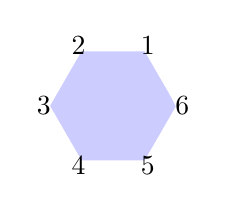
\begin{tikzpicture}
\newdimen\Radi
\Radi=0.8cm
    % Indicate the boundary of the regular polygons
%    \draw [thin,black!20] circle (\R) ;
%    \fill[black!20] circle (2pt);
%    \draw (0:\R) \foreach \x in {120,240} {
%            -- (\x:\R)
%        } -- cycle (90:\R) node[above] {$n=3$} ;
%    \draw[xshift=2.5\R] (0:\R) \foreach \x in {90,180,...,359} {
%            -- (\x:\R)
%        } -- cycle (90:\R) node[above] {$n=4$} ;
%    \draw[xshift=5.0\R] (0:\R) \foreach \x in {72,144,...,359} {
%            -- (\x:\R)
%        } -- cycle (90:\R) node[above] {$n=5$} ;
    \begin{scope}[yshift=-3\Radi]
        \fill[blue!20] (0:\Radi) \foreach \x in {1,...,6} { %60,120,...,359} {
                -- ({60*\x}:\Radi)
            }-- cycle (90:\Radi); % node[above] {$n=6$} ;
        \draw[white] (0:\Radi) \foreach \x in {1,...,6} { %60,120,...,359} {
                -- ({60*\x}:{1.1*\Radi}) node[black] {$\x$}
            }-- cycle (90:\Radi); % node[above] {$n=6$} ;
            
%        % 360/7 = 51.4286 For PGF v < 1.18 we have to round to the nearest
%        % integer. Newer version support fractional angle values.
%        % For a more accurate result use the sequence
%        % {51, 103, 154, 206, 257, 309}
%        %
%        \draw[xshift=2.5\R] (0:\R) \foreach \x in {51.4286,102.8571,...,359} {
%                -- (\x:\R)
%            }-- cycle (90:\R) node[above] {$n=7$} ;
%        \draw[xshift=5.0\R] (0:\R) \foreach \x in {45,90,...,359} {
%                -- (\x:\R)
%            } -- cycle (90:\R) node[above] {$n=8$} ;
    \end{scope}
%    \draw[yshift=-6.0\R] (0:\R) \foreach \x in {10,20,...,359} {
%            -- (\x:\R)
%        } -- cycle (90:\R) node[above] {$n=36$} ;
\end{tikzpicture}
\end{document}
